\section{Data-Driven Turbulence Modeling}
\label{sec:turbulence}


\subsection{Governing Equations}
\label{sec:equations}
The temporal evolution of compressible, viscous flows is described by the Navier-Stokes equations, which can be written as
\begin{equation}
  U_t + \nabla_x\cdot \left(F^c - F^v\right) = 0,
  \label{eq:navier_stokes}
\end{equation}
with $U=\left(\rho, \rho v_1, \rho v_2, \rho v_3, \rho e \right)^T$ as the vector of conserved quantities comprising density, the three-dimensional momentum vector and energy, respectively.
Here, $(\cdot)_t$ indicates the differentiation with respect to time and the nabla operator $\nabla_x$ the differentiation with respect to the three Cartesian coordinates $x_i$ with $i=1,2,3$.
The convective flux $F^c$ and the viscous flux $F^v$ with columns $i=1,2,3$ can be written as 
\begin{equation}
  F_i^c =
  \left(
  \begin{array}{c}
    \rho v_i \\
    \rho v_1 v_i + \delta_{1i} p\\
    \rho v_2 v_i + \delta_{2i} p\\
    \rho v_3 v_i + \delta_{3i} p\\
    \rho e v_i + p v_i
  \end{array}
  \right)
  ,\;
  F_i^v =
  \left(
  \begin{array}{c}
    0 \\
    \sigma_{1i}\\
    \sigma_{2i}\\
    \sigma_{3i}\\
    \sigma_{ij}v_j-q_i
  \end{array}
  \right) ,
  \label{eq:fluxes_written_out}
\end{equation}
where $p$ denotes the pressure and $\delta_{ij}$ is the Kronecker delta.
The three-dimensional velocity vector is given by $v =(v_1,v_2,v_3)^T$.
The stress tensor $\sigma_{ij}$ and the heat flux $q_i$ can be written as
\begin{align}
  \sigma_{ij} &= \mu\left(\frac{\partial v_i}{\partial x_j}+\frac{\partial v_j}{\partial x_i}-\frac{2}{3}\delta_{ij}\frac{\partial v_k}{\partial x_k}\right) ,
  \label{eq:stress_tensor}\\
  q_i &= - \kappa\:\frac{\partial T}{\partial x_i},
  \label{eq:heat_flux}
\end{align}
with $\mu$ as the viscosity and $\kappa$ as the heat conductivity.
The equations are closed with the ideal gas assumption, which yields the equation of state as
\begin{equation}
  p = \left(\frac{c_p}{c_v}-1\right) \left(\rho e-\frac{\rho}{2}\left(v_1^2+v_2^2+v_3^2\right)\right),
\end{equation}
with $c_p$ and $c_v$ as the specific heats.
In the following, the Navier-Stokes equations are always solved in the incompressible limit with a Mach number of $\mathrm{Ma}=0.1$.



\subsection{Forced Homogeneous Isotropic Turbulence}

\begin{figure}
  \begin{minipage}[t]{0.443\linewidth}
    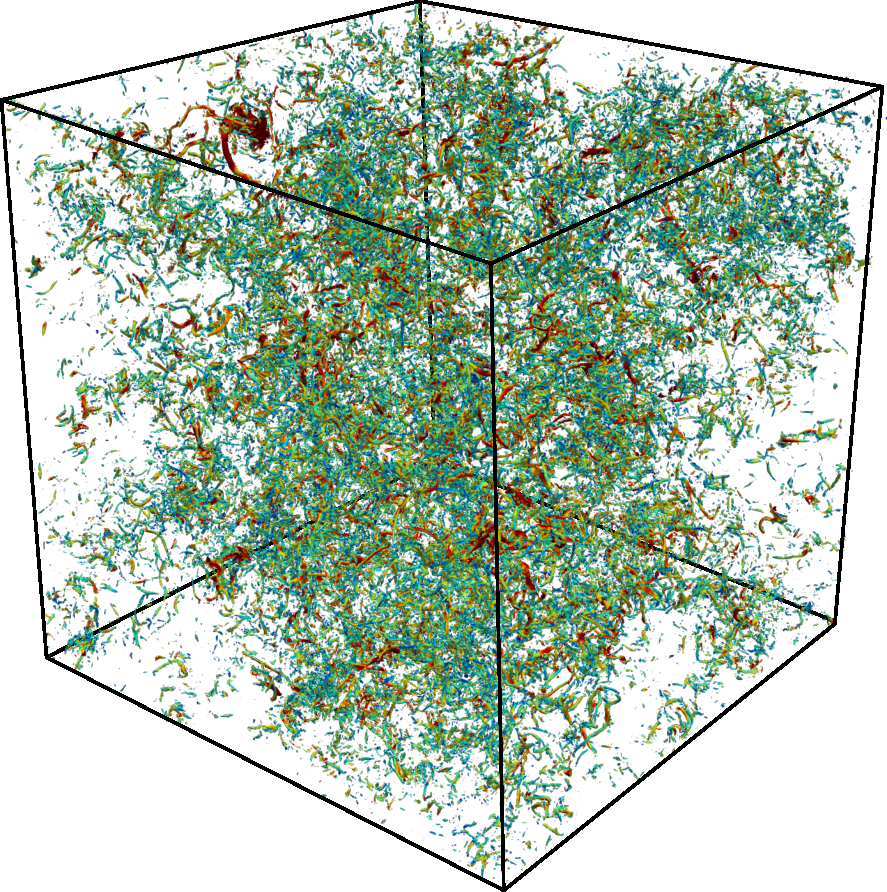
\includegraphics[width=\linewidth]{./fig/HIT.pdf}%
  \end{minipage}
  \hfill
  \begin{minipage}[t]{0.53\linewidth}
    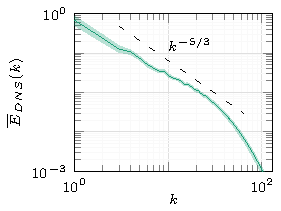
\includegraphics[width=\linewidth]{./tikz_double_column/draft-figure0.pdf}%
  \end{minipage}
  \caption{Instantaneous flow field of the HIT test case visualized with iso-surfaces of the Q-criterion colored by the velocity magnitude (left) and the mean spectrum of the kinetic energy for the DNS of a forced HIT over the wavenumbers $k$ (right). The shaded area indicates the maximum and minimum observed energy of the corresponding wavenumber.}
  \label{fig:HIT}
\end{figure}

Homogeneous isotropic turbulence (HIT) is a canonical test case for turbulent flows and can be considered as \textit{turbulence-in-a-box}.
The HIT test case describes freely evolving turbulence without an imposed mean flow, influences of walls or any external driving forces.
The computational domain is typically a cube with periodic boundary conditions, as illustrated in \figref{fig:HIT}, which is discretized by an equidistant Cartesian mesh.
The domain is initialized with an initial velocity field that obeys a given turbulence spectrum and is divergence-free.
In this work, the initial flow state was obtained by Rogallo's procedure \cite{Rogallo1981}.
Over time, the flow then produces a turbulent energy spectrum as shown in \figref{fig:HIT}.
In turbulence, energy is transported in the mean from the large scales to the small scales, where the energy is dissipated by the viscosity of the fluid.
In the absence of large scale shear and due to this dissipation mechanism, the velocity fluctuations decrease over time and tend towards zero.
Therefore, this flavor of the HIT test case is also referred to as decaying HIT.
However, this transient behavior causes the flow and the turbulent statistics to change continuously over time.

Different forcing strategies are proposed in literature to inject the dissipated energy back into the system and thus sustain the turbulent flow.
This allows to obtain a turbulent flow with stationary statistics.
For methods with a globally defined solution basis, the forcing can be added in the low modes only, while the higher wavenumbers remain unaffected.
For discretizations with a local basis with compact support, e.g. finite-volume or discontinuous Galerkin schemes, the global Fourier modes of the solution are generally unknown and costly to evaluate.
Instead, a nodal forcing is applied, which acts directly on the solution points instead of global wavenumbers.
Since in this approach the forcing is not limited to the low wavenumbers, the forcing adds energy across the whole spectrum.
This causes the slope in \figref{fig:HIT} to slightly deviate from its theoretical $k^{-5/3}$ trend, since this influx of energy into the high wavenumber modes is not optimal. %
We point out however that, first, such a nodal forcing is often used in element-based discretization schemes and, second, the results in \figref{fig:HIT} indicate that the unwanted effects are minimal.

In this work, we apply the linear isotropic forcing method proposed by Lundgren in \cite{lundgren2003linearly} and analyzed further in \cite{de2015anisotropic}.
Here, a forcing term $f$ is added to \eqref{eq:navier_stokes}, which yields
\begin{equation}
  U_t + \nabla_x\cdot \left(F^c - F^v\right) = f.
  \label{eq:forced_navier_stokes}
\end{equation}
For isotropic forcing, the forcing is assumed to be parallel to the current momentum vector, which gives
\begin{equation}
  f = Q \: 
  \left(
  \begin{array}{c}
    0 \\
    \rho v\\
    0
  \end{array}
  \right),
\end{equation}
where $Q$ is a scalar that quantifies the difference between the current kinetic energy in the flow $E=\frac{\rho}{2} (v\cdot v)$ integrated over the domain and the prescribed target value.
In our implementation, a single forcing parameter $Q$ is employed for the whole flow domain.


\subsection{Large Eddy Simulation}
\label{sec:les}


\begin{figure}[tb]
  \centering
  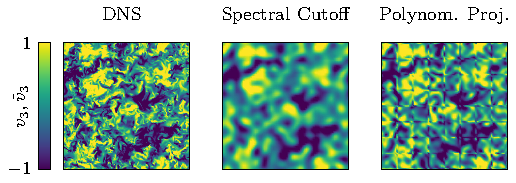
\includegraphics[width=0.99\linewidth]{tikz_double_column/draft-figure1.pdf}
  \caption{Slices of the instantaneous velocity field of homogeneous isotropic turbulence. The LES flow fields are obtained from the DNS field (left) by applying a spectral cutoff filter (middle) or a projection filter onto a piecewise polynomial basis (right). The latter explicit LES filter can be seen as a rough approximation of the unknown implicit filter form of the DG scheme. More details on the LES filters are given in \cite{kurz2022machine}.}
  \label{fig:les_filter}
\end{figure}

For most flows, it is computationally intractable to resolve all length scales present in the flow.
Instead, the simulation resolves only the largest flow scales, which contain the majority of the kinetic energy.
This approach is referred to as large eddy simulation (LES).
This corresponds to applying a low-pass filter $\tilde{(\cdot)}$ to the governing equations in \eqref{eq:navier_stokes} and solving the resulting evolution equation for the coarse-scale solution $\tilde{U}$.
In \figref{fig:les_filter}, we apply known filter kernels in an a priori manner to visualize the resulting solution fields.
Due to the non-linearity of the governing equations, the filtering operation introduces additional terms into the equation, which describe the effect of the non-resolved fine scales onto the resolved large scales.
These closure terms rely on the full solution $U$ and are thus generally unknown causing the closure problem of LES.
Therefore, a suitable turbulence model is employed that attempts to approximate the unknown closure terms based on the coarse-scale solution $\tilde{U}$.

From \figref{fig:les_filter} we can already appreciate the fact that the associated closure terms will be a function of the chosen filter.
In practice however, the filtering operation is typically not given by means of an explicit filter function.
Instead, the underresolved discretization acts as an implicit LES filter.
While this allows to incorporate all wavenumbers within the resolution limits of the underlying discretization into the simulation and thus improves the efficiency of the LES, the form of the LES filter $\tilde{(\cdot)}$ is generally unknown.
As a consequence, the closure terms for implicitly filtered LES cannot be computed, even if the full solution $U$ is available, since this would require to apply the unknown implicit LES filter, i.e. an application of the spatial and temporal operators.
This makes model development difficult, since the models cannot be optimized by simply fitting them to the \textit{exact} closure terms computed from high-fidelity data.

A common modeling strategy is to mimic the energy transport from the large to the small scales in turbulent flows by introducing a turbulent viscosity.
For instance, Smagorinsky's model \cite{smagorinsky1963general} computes this viscosity as 
\begin{equation}
  \mu_t = \rho\left(C_s\,\Delta\right)^2 \sqrt{2\,\tilde{S}_{ij}\,\tilde{S}_{ij}} \quad \text{with}\quad \tilde{S}_{ij}=\frac{1}{2}\left(\frac{\partial \tilde{v}_i}{\partial x_j}+\frac{\partial \tilde{v}_j}{\partial x_i}\right),
  \label{eq:smago}
\end{equation}
where $\tilde{S}_{ij}$ is the resolved rate-of-strain tensor, $\Delta$ is the filter width of the LES filter and $C_s$ is a model parameter, which has to be tuned manually to specific flows and discretizations.
The eddy-viscosity methodology has the advantage that the LES equations for the coarse-scale solution 
\begin{equation}
  \tilde{U}_t + \nabla_x\cdot \left(\tilde{F}^c - \tilde{F}^v_{turb}\right) = \tilde{f},
  \label{eq:les_equation}
\end{equation}
look identical to forced Navier-Stokes equations in \eqref{eq:forced_navier_stokes}.
Only the viscous flux $\tilde{F}^v_{turb}$ is modified slightly by adding the turbulent viscosity $\mu_t$ to the physical one.
Another common approach is the implicit modeling strategy.
Here, it is acknowledged that the employed discretization adds numerical dissipation to the system which can be interpreted as an implicit turbulence model.

In the standard Smagorinsky model (SSM), the parameter $C_s$ is constant in the computational domain and has to be chosen a priori.
So-called dynamic models alleviate these restrictions by adapting their model parameters based on the current flow state dynamically in space and time.
This concept gives rise to the dynamic Smagorinsky model (DSM), which is detailed in \ref{app:dynsmago}.
In the following, we strive to enhance the Smagorinsky model by means of our RL framework by training an agent to dynamically adapt the model coefficient in space in time during the LES, i.e $C_s=C_s(x_i,t)$.




\subsection{Reinforcement Learning for Turbulence Modeling}


\begin{table*}[htb!]
  \begin{tabularx}{1.0\linewidth}{p{0.125\textwidth}p{0.175\textwidth}X}
    \toprule
    Symbol & Meaning & Turbulence Modeling \\
    \midrule
    $\states$                  & Environment states    & Current flow state of the LES $\tilde{U}$ from which the policy's inputs can be computed.\\
    $\actions$                 & Agent's action space  & Elementwise parameter for Smagorinsky's model within $C_s \in[0,0.5]$ (\figref{fig:policy}).\\
    $\sgeneralpolicy$          & Agent's policy        & CNN-based architecture with elementwise inputs and outputs (\figref{fig:policy}).\\
    $\sgeneraltransition$      & Transition function   & Integration of LES equations, \eqref{eq:les_equation}, for current predictions of $C_s$.\\
    $\rewardfunc(s_t,s_{t+1})$ & Reward function       & Based on error in turbulent energy spectra compared to DNS solution, \eqref{eq:reward}.\\
    \bottomrule
  \end{tabularx}
  \caption{Definition of the major building blocks for the formulation of turbulence modeling as a Markov decision process, as given in \figref{fig:MDP}.}
  \label{tab:rl_turb}
\end{table*}


\begin{figure*}[htb]
  \centering
  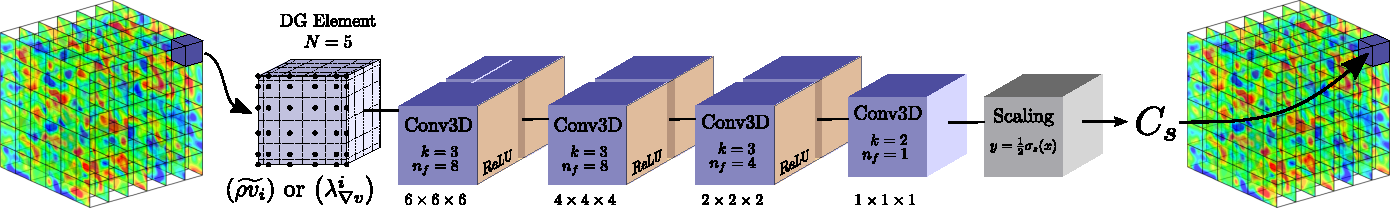
\includegraphics[width=0.99\textwidth]{./fig/DGnet.pdf}
  \caption{Network architecture of the CNN-based policy network for $N=5$. The inputs of the network are either the momentum field $(\widetilde{\rho v}_1,\widetilde{\rho v}_2,\widetilde{\rho v}_3)^T$ or the five invariants of the velocity gradient tensor $\lambda_{\nabla v}^i$ in a single DG element with given $N$, for which the distribution of interpolation points is shown exemplarily. The network comprises several three-dimensional convolutional layers (Conv3D) with the corresponding kernel sizes $k$ and the number of filters per layer $n_f$. The output sizes in the dimensions of convolution are given below each layer. The first layer retains the input dimension by means of zero-padding, while for the other layers no padding is employed in order to retain a scalar output $C_s$ per element. The scaling layer applies the sigmoid activation function $\sigma_s(x)$ in order to scale the network output to $C_s\in [0,0.5]$ and can be interpreted as the activation function of the last layer.}
  \label{fig:policy}
\end{figure*}


The problem of turbulence modeling has to be framed as an MDP in order to solve it within the RL framework, as already discussed in \secref{sec:rl}.
In the following, we use LES of forced HIT as the training environment for the agent.
The agent interacts with the environment by adapting the model coefficient of \eqref{eq:smago} dynamically in space in time for each element. %
We use a policy based on convolutional ANN (CNN) to account for the non-locality of turbulence.
To this end, the policy takes the flow state in a single element as input and predicts a single $C_s$ parameter for the respective element as output, as illustrated in \figref{fig:policy} for $N=5$.
The sigmoid function is applied to the output of the ANN to scale the prediction to $C_s\in[0,0.5]$.
Since only $C_s^2$ is used in Smagorinsky's model in \eqref{eq:smago}, we avoid negative predictions to preserve a monotonous relationship between the prediction and the actual eddy-viscosity introduced in the flow.
This choice was made to stay true to the original idea of Smagorinsky's model.
The upper limit is selected generously, while retaining the predictions in a sensible range to accelerate training.%
\footnote{It was verified for selected training configurations that the agent reaches similar levels of accuracy if the limits are omitted, i.e. $C_s\in(-\infty,\infty)$. However, the agent requires much more training iterations in this case than with the scaling applied.}

The states $\states$ are represented by the vector of conserved quantities $\tilde{U}$ on the coarse LES mesh, which gives a complete description of the current flow state.
Based on this state, two different sets of input quantities are investigated for the policy.
First, we use the elementwise three-dimensional momentum field as input, i.e. the vector $(\widetilde{\rho v}_1,\widetilde{\rho v}_2,\widetilde{\rho v}_3)^T$.
While this is a common choice in ANN-based turbulence modeling, the momentum field lacks invariance with respect to scaling and rotation.
To this end, we also investigate the input features proposed by Novati et al. \cite{novati2021automating}, who used as input quantities the five invariants of the velocity gradient tensor $\lambda_{\nabla v}^i$, as given by Pope in \cite{pope1975more}, to embed Galilean invariance into their policy.

It is important to stress that in contrast to previous works, our policy acts on \textit{local} inputs only.
This means that the predictions for each element are based solely on the flow state inside of this respective element.
The predictions for each individual element are thus independent from the remaining flow field and do not require any information about the global flow state.
This makes this approach more suitable for realistic applications, where global flow statistics are generally very expensive to retrieve during runtime.
Moreover, models which rely on global flow statistics as inputs cannot be evaluated on flows where these statistics cannot be obtained in a straight-forward manner, e.g. due to the geometric complexity of the computational domain or where a global statistic simply does not exist.
The value network is designed analogously to the policy network, but employs two additional fully-connected layers, comprising 16 and a single neuron, respectively, to combine the elementwise predictions for the whole flow state to a single prediction for the state-value function.
This RL design can be interpreted as a multi-agent RL approach, where each element employs its own agent, but all agents share their weights.
Given the predictions of the policy, i.e. the actions of the agent, the new state of the environment is obtained by integrating the LES equations in time for $\Delta t_{RL}$. 

As overall optimization target of the RL task, we define the error in the spectrum of turbulent kinetic energy between the instantaneous LES $E_{LES}$ and the target spectrum $\overline{E}_{DNS}$.
In this work, we used the time-averaged spectrum of a previously computed DNS.
However, the RL framework allows to impose any high-level statistic as training objective.
To this end, also data reported in the literature, experimental data or even physical properties like the $k^{-5/3}$ energy decay in the inertial range could be used directly as optimization targets. 
Given these energy spectra, we compute the mean squared error for the wavenumbers $k$ up to $k_{max}$.
Here, $k_{max}$ is the maximum wavenumber considered for optimization and thus depends on the employed resolution of the LES.
Finally, we use the exponential function to normalize the resulting reward to the range $[-1,1]$, since a normalized reward can improve the training speed.
The reward function thus reads
\begin{equation}
  \rewardfunc(\state) = 2\:\exp\left(-\frac{1}{\rewardscale\:\wavenumber_{max}}\sum_{\wavenumber=1}^{\wavenumber_{max}}\left(\frac{\overline{\turbenergy}_{DNS}(\wavenumber)-\turbenergy_{LES}(\wavenumber)}{\tfilter{\turbenergy}_{DNS}(\wavenumber)}\right)^2\right)-1,
  \label{eq:reward}
\end{equation}
with $\alpha$ as a scaling factor.
This scaling factor controls the difficulty of the training task by balancing between providing the maximum reward for any action of the policy for $\alpha \rightarrow \infty$ and demanding impossible accuracy in the spectrum to escape the negative limit of the exponential function for $\alpha \rightarrow 0$.
It seems important to stress that the energy spectra only have to be computed to evaluate the reward function during training and are not required if the trained policy is later applied in practical simulations.
The proposed formulation of turbulence modeling as an MDP is summarized in \tabref{tab:rl_turb}.

A major advantage of the broader learning paradigm of RL in comparison to the common SL approach is that RL allows to incorporate a much broader range of prior information into the training.
The optimization target for the training, which is defined via the reward function, can be based on DNS data, experimental data, physical first principles or properties of the underlying discretization.
For SL, any change in the posed learning task, e.g. changing the input and output quantities for the ANN, would require to recompute the training dataset from DNS data.
This poses significant challenges, since it requires to store and process large amounts of time-resolved DNS data.



\subsection{Computational setup}
\label{sec:relexi}


\begin{table}[htb]
  \centering
  \begin{tabular}{lrrrr}
    \toprule
    Name   & $N$ & \#Elems & $k_{max}$ & $\alpha$ \\
    \midrule
    24 DOF &   5 &   $4^3$ &         9 &      0.4 \\
    32 DOF &   7 &   $4^3$ &        12 &      0.4 \\
    36 DOF &   5 &   $6^3$ &        13 &      0.4 \\
    48 DOF &   5 &   $8^3$ &        16 &      0.4 \\
    \bottomrule
  \end{tabular}
  \caption{Investigated configurations for the LES environments. The names are derived from the number of degrees of freedom (DOF) in each direction used for the simulation, which can be computed as the number of elements in each direction times $(N+1)$.}
  \label{tab:les_configs}
\end{table}

In RL, the training of the agent is an iterative process which does not require the perfect target quantities to be known, but finds suitable targets by itself in order to fulfill the overall goal defined by the reward function.
This means that no DNS data is required to compute input and output data pairs for a training dataset.
Instead, a number of LES runs has to be computed repeatedly to sample interactions between the agent and the environment.
Thus, like in most ML methods, training requires considerable hardware resources for running the LES and training the agent on the collected experience.
In this work, we use the Relexi framework proposed in \cite{kurz2022deep,kurz2022relexi} to train the agent by using the parallel computing resources provided by today's high-performance computing (HPC) systems.
The Relexi framework implements the RL training loop by means of the TensorFlow library \cite{abadi2016tensorflow} and its RL extension TensorFlow-Agents \cite{TFAgents}.
The framework allows to couple external flow solvers efficiently on high-performance computing systems with the SmartSim library \cite{partee2021using}, which is used to manage the simulations runs and implements the communication between the main application and the external solver.
The LES environments are simulated with the HPC flow solver FLEXI \cite{krais2021flexi}.
In each training iteration, Relexi starts several FLEXI simulations to sample interactions of the current policy with the LES environments.

With FLEXI we employ a high-order discontinuous Galerkin (DG) discretization of the compressible Navier-Stokes equations using a kinetic energy preserving split formulation of the fluxes on Legendre-Gauss-Lobatto interpolation nodes for stability as discussed by Flad and Gassner in \cite{flad2017use}.
We investigate the influence of the discretization on the RL agent by computing LES at different resolutions as listed in \tabref{tab:les_configs}.
For this, we also employ two different polynomial degrees, i.e. $N=5$ and $N=7$, which results in two different discretizations. 
The maximum wavenumber used for optimization $k_{max}$ is then chosen for each case according to the respective resolution employed.
Theoretically, a minimum of $n_{ppw}=\pi$ points per wavelength is required to resolve a wavenumber accurately with a polynomial basis.
For the polynomial degrees employed here, the resolution capabilities can be estimated as $n_{ppw}\approx 4$ \cite{gassner2011comparison}.
However, to increase the difficulty of the optimization task, we choose $k_{max}$ such that $2.6 \le n_{ppw} \le 3$.
This forces the RL algorithm to optimize over all represented wavenumbers.
 
All simulations are initialized with flow states that are obtained by projecting the high-fidelity DNS solution, which is obtained a priori, onto the resolution of the respective environment using an $L_2$-projection.
The forced HIT case has a Reynolds number of $\mathrm{Re}_{\lambda}\approx 180$ with respect to the Taylor microscale.
The initial states used for training are drawn from the filtered DNS evaluated at $t_{DNS}=3,4,5,6$ and a single flow state at $t_{DNS}=8$ is kept hidden for testing, i.e. to evaluate the policy's performance on unseen data.
The LES are then simulated for $\Delta t_{end}=5$ using the FLEXI solver, while the elementwise $C_s$ parameters are updated every $\Delta t_{RL}=0.1$.
The large-eddy turnover time with approximately $t'\approx 0.7$ acts as a characteristic timescale, which results in 7 characteristic timescales simulated in each LES run.
This is considered sufficient to incorporate long-term effects into the training process.

For the RL algorithm, we use the Adam optimizer \cite{kingma2014adam} with a learning rate of $10^{-4}$ for the policy and the value network.
All configurations were trained for 5 epochs in each training iteration, except the 48 DOF configuration, which was only trained for a single epoch.
Instead of using mini-batching, the gradients were computed with respect to all sampled experience.
The weighting factor between the policy and the value estimation loss is set to 0.5 and the clipping parameter to $\ppoclipping=0.2$.
No additional regularization was used and the originally proposed entropy regularization coefficient for PPO is set to zero.
Moreover, we chose a discount factor of $\gamma=0.995$.
To obtain stochastic predictions from the deterministic policy, we sample actions from a normal distribution which is determined by using the ANN's predictions as mean and a fixed standard deviation of 0.02, which corresponds to about 10\% of the theoretical $C_s=0.17$ suggested for Smagorinsky's model in the literature.
